\documentclass[11pt,
  paper=a4, 
  bibliography=totocnumbered,
	captions=tableheading,
	BCOR=10mm
]{scrreprt}

\usepackage[utf8]{inputenc}
 
 
\usepackage[onehalfspacing]{setspace}
\usepackage{csquotes} % Context sensitive quotation.
\usepackage{amsmath} % Standard math.
\usepackage{amsthm} % Math theorems.
\usepackage{amssymb} % More math symbols.
\theoremstyle{definition}
\newtheorem{definition}{Definition}[chapter]
 
\usepackage[section]{placeins} % Keep floats in the section they were defined in.
\usepackage{tabularx}
\usepackage{booktabs} % Scientific table styling.
\usepackage{floatrow} % Option for keeping floats in the place they were defined in the code.
\floatsetup[table]{style=plaintop}
\usepackage{hyperref} % Hyperlinks.
\usepackage[all]{nowidow} % Prevent widows and orphans.
\usepackage{xstring} % logic string operations
\usepackage[nopostdot, nonumberlist]{glossaries} % glossary for definitions and acronyms, without dot after entry and page reference 
\usepackage{bbm} % \mathbb on numerals.
\usepackage{csquotes}
\usepackage{mathtools}
\usepackage[ruled,vlined]{algorithm2e} %Pseudocode
\usepackage{scrhack} % Make warning go away.
\usepackage{graphicx}
\usepackage{subcaption} % Subfigures with subcaptions.
\usepackage{authoraftertitle} % Make author, etc., available after \maketitle
\usepackage{listofitems}
\usepackage{blindtext} % Placeholder text.
\usepackage[nopostdot, nonumberlist]{glossaries}
\makeglossaries % Generate the glossary

% \PassOptionsToPackage{obeyspaces}{url}%
\usepackage[backend=bibtex,% 
style=nature,% 
doi=true,isbn=false,url=false, eprint=false]{biblatex}
% \renewbibmacro*{url}{\printfield{urlraw}}

\addbibresource{bib/library.bib}

\DeclareStyleSourcemap{
  \maps[datatype=bibtex, overwrite=true]{
    \map{
      \step[fieldsource=url, final]
      \step[typesource=misc, typetarget=online]
    }
    \map{
      \step[typesource=misc, typetarget=patent, final]
      \step[fieldsource=institution, final]
      \step[fieldset=holder, origfieldval]
    }
  }
}

%\linespread{1.5} % set line spacing
 
\usepackage{listings} % rendering program code
\lstset{% general command to set parameter(s)
	basicstyle=\ttfamily\color{grey},          % print whole listing small
	keywordstyle=\color{black}\bfseries\underbar,
	% underlined bold black keywords
	identifierstyle=,           % nothing happens
	commentstyle=\color{white}, % white comments
	stringstyle=\ttfamily,      % typewriter type for strings
	showstringspaces=false}     % no special string spaces


\DeclareFontFamily{U}{mathx}{\hyphenchar\font45}
\DeclareFontShape{U}{mathx}{m}{n}{
      <5> <6> <7> <8> <9> <10>
      <10.95> <12> <14.4> <17.28> <20.74> <24.88>
      mathx10
      }{}
\DeclareSymbolFont{mathx}{U}{mathx}{m}{n}
\DeclareFontSubstitution{U}{mathx}{m}{n}
\DeclareMathSymbol{\bigtimes}{1}{mathx}{"91}

 

%%% Custom definitions %%%
% Shorthands
\newcommand{\ie}{i.\,e.~}
\newcommand{\eg}{e.\,g.~}
\newcommand{\ind}{\mathbbm{1}}
% Functions
\newcommand{\tpow}[1]{\cdot 10^{#1}}
\newcommand{\figref}[1]{(Figure \ref{#1})}
\newcommand{\figureref}[1]{Figure \ref{#1}}
\newcommand{\tabref}[1]{(Table \ref{#1})}
\newcommand{\tableref}[1]{Table \ref{#1}}
\newcommand{\secref}[1]{%
	\IfBeginWith{#1}{chap:}{%
		(cf. Chapter \ref{#1})}%
		{(cf. Section \ref{#1})}%
		}
\newcommand{\sectionref}[1]{%
	\IfBeginWith{#1}{chap:}{%
		Chapter \ref{#1}}%
		{\IfBeginWith{#1}{s}{%
			Section \ref{#1}}%
			{[\PackageError{sectionref}{Undefined option to sectionref: #1}{}]}}}
\newcommand{\chapref}[1]{(see chapter \ref{#1})}
\newcommand{\unit}[1]{\,\mathrm{#1}}
\newcommand{\unitfrac}[2]{\,\mathrm{\frac{#1}{#2}}}
\newcommand{\codeil}[1]{\lstinline{#1}}{} % wrapper for preventing syntax highlight error
\newcommand{\techil}[1]{\texttt{#1}}
\newcommand{\Set}[2]{%
  \{\, #1 \mid #2 \, \}%
}
% Line for signature.
\newcommand{\namesigdate}[1][5cm]{%
	\vspace{5cm}
	{\setlength{\parindent}{0cm}
	\begin{minipage}{0.3\textwidth}
		\hrule 
		\vspace{0.5cm}
		{\small city, date}
	\end{minipage}
	 \hfill
	\begin{minipage}{0.3\textwidth}
		\hrule
		\vspace{0.5cm}
	    {\small signature}
	\end{minipage}
	}
}
% Automatically use the first sentence in a caption as the short caption.
\newcommand\slcaption[1]{\setsepchar{.}\readlist*\pdots{#1}\caption[{\pdots[1].}]{#1}}

% Variables. 
% Adapt if necessary, use to refer to figures and graphics.
\def \figwidth {0.9\linewidth}
\graphicspath{ {./graphics/figures/}{./graphics/figures/} } % Path to figures and images.


% Customizations of existing commands.
\renewcommand{\vec}[1]{\mathbf{#1}}
% Capitalized \autoref names.
\renewcommand*{\chapterautorefname}{Chapter}
\renewcommand*{\sectionautorefname}{Section}


% TODO Fill with your data.
\title{Image Segmentation}
\author{Sven Groen}

\begin{document}

\begin{titlepage}
	\begin{flushleft}
		Universität Osnabrück\\
		Fachbereich Humanwissenschaften\\
		Institute of Cognitive Science
	\end{flushleft}

	\vspace{2cm}
	\centering{
		Bachelorthesis - Expose \vspace{1cm}\\
		\textbf{\Large{\MyTitle}}
		\vspace{1cm}\\
		\begin{tabular}{c}
			\MyAuthor                          \\
			970219                            \\
			Bachelor's Program Cognitive Science \\
			Starting month and year - end month and year
		\end{tabular}}
	\vspace{1cm}

	\begin{tabular}{ll}
		First supervisor:  & Manuel Kolmet          \\
		                   & IMANOX GmbH             \\
		                   & Berlin                   \\\\
		Second supervisor: & Prof. Dr. Someone Else         \\
		                   & Institute of Cognitive Science \\
		                   & Osnabrück
	\end{tabular}

\end{titlepage}


\pagenumbering{gobble}
\pagebreak


\tableofcontents
\listoffigures
\listoftables
\listofalgorithms


\chapter{Goal and background information}
\pagenumbering{arabic}

\section{Cooperation with Imanox}
This project is realized in cooperation with \href{https://www.imanox.de/}{Imanox} . 
Imanox is a Berlin-based Startup that developed a smart photo booth for expositions, events and promotions. 
This photo booth enables customers virtual product placements using augmented and mixed reality. 
Main features are hand-tracking, digital masks and changing virtual backgrounds.

\section{Virtual backgrounds}
Currently, the photo booth has a build in depth sensor that measures the distance of objects by casting illumination onto the scene and indirectly measuring the time it takes to travel back to the camera. 
The camera struggles with correctly predicting the depth in certain situations. 
Pixels are rendered as invalid and no depth information is provided. 
The reasons for this are numerous. 
Pixels might get under saturated (signal is not strong enough) or over saturated (signal is too strong). 
Other artifacts occur due to the geometry of the scene. 
The sensors of the camera might receive signals from multiple locations in the scene, leading to an ambiguous depth. 
Especially around the edges and borders of objects pixels contain mixed signals from fore-and background leading to blurred outlines.
In the current version of the photo booth alpha values (0 to 1) are calculated based on the data from the depth sensor. 
Objects in the foreground receive high alpha values and the background is considered to have an alpha value of 0, making it transparent. 
In this way the background can be virtually replaced without affecting the objects in the foreground. 
Due to the described inaccurate data that is given by the depth sensor the result is of low quality. 
The edges and borders of the objects/people in the scene are not sharp and often misclassified. 
Especially for small / thin objects, \eg hair, the camera hardly recognizes it and parts of the hair are therefore considered as background and are also replaced by the virtual background.
For more detailed information on this issue I refer to \url{https://docs.microsoft.com/de-de/azure/Kinect-dk/depth-camera}.
\cite{Microsoft2019}

\section{Goal of the thesis}
The goal of this bachelor thesis is to improve the quality of the semantic segmentation of the current Imanox photo booth using machine learning techniques.
We will use ...

\chapter{Segmentation}
\textcite{Szeliski2011} refers to image segmentation as "the task of finding groups of pixels that 'go together' " (p. 237).
In the following semantic segmentation refers to a pixel-wise classification of an image \cite{Mittal2020}.
In the classical image classification tasks the task is to name the objects that can be seen in an image.
Semantic segmentation extends this problem further. 
Each pixel in an image is assigned to one category label given a set of categories.
However, individual instances of an object in one image are not differentiated.
When individual instances in an image should be recognized, object detection is necessary.
For single objects this would be a classification + localization task. 
Object detection is usually realized by framing the object with a box and assigning a category label to each box.
Lastly, there is instance segmentation. 
Instance segmentation extends the problem of object detection by a pixel-wise classification (similar to semantic segmentation) but with instances being differentiated \cite{Mittal2020}.
See \figref{fig:Computer_Vision_Tasks} for an overview of the described tasks.
Given the goal of this project only semantic segmentation is necessary.
Detailed information which objects are in the scene is not required.
\begin{figure}[H]
	\centering
	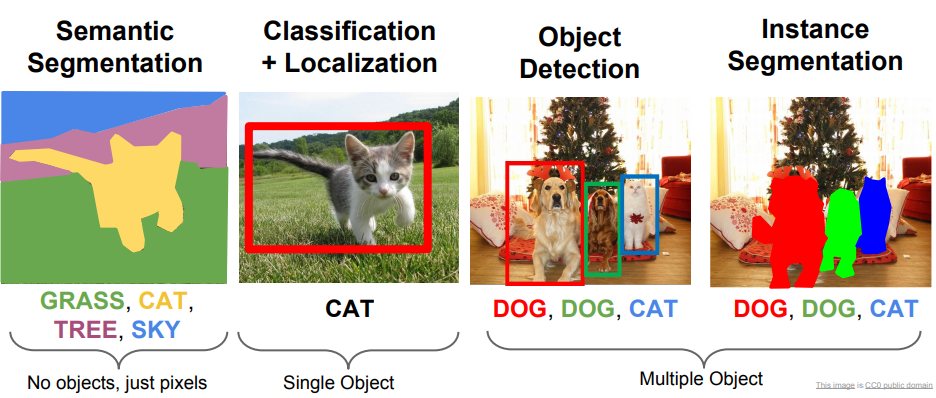
\includegraphics[width=\figwidth]{Computer_Vision_Tasks}
	\slcaption{
		Overview of Computer Vision Tasks. (\textcite{Fei-Fei2017}, Slide 17).
		\label{fig:Computer_Vision_Tasks}}
\end{figure}

\section{related work}

Segmenting an image into its individual parts is a classical problem of computer vision \cite{Szeliski2011}. 
Early methods involve classical methods like threshold detection \cite{Smith1979}, while modern approaches like k-means clustering \cite{Dhanachandra2015} improved the results.
Deep learning architectures, especially convolutional neural networks (CNNs) \cite{Fukushima1980}, have lead to an improvement in performance whereas classical methods have seem to reach a plateau \figref{fig:Object_Detect_impact_of_DL}.
\textcite{Shelhamer2017} have been the first to proposed a CNN architecture where a pixel-wise supervised training was achieved. 
This was done by upsampling the class prediction layer to the input image size, leading to a pixel-wise classification.
Following papers proposed different architectures. \textcite{Chen2018} proposed a combination of Deep CNNs with fully connected conditional random fields (CRFs) that tries to grasp the semantic context of the image.
\textcite{Noh2015} suggested a "Deconvolutional Network" with special unpooling and deconvolution operations.
A similar Encoder-Decoder architecture has been proposed by \textcite{Badrinarayanan2017}.



\begin{figure}[H]
	\centering
	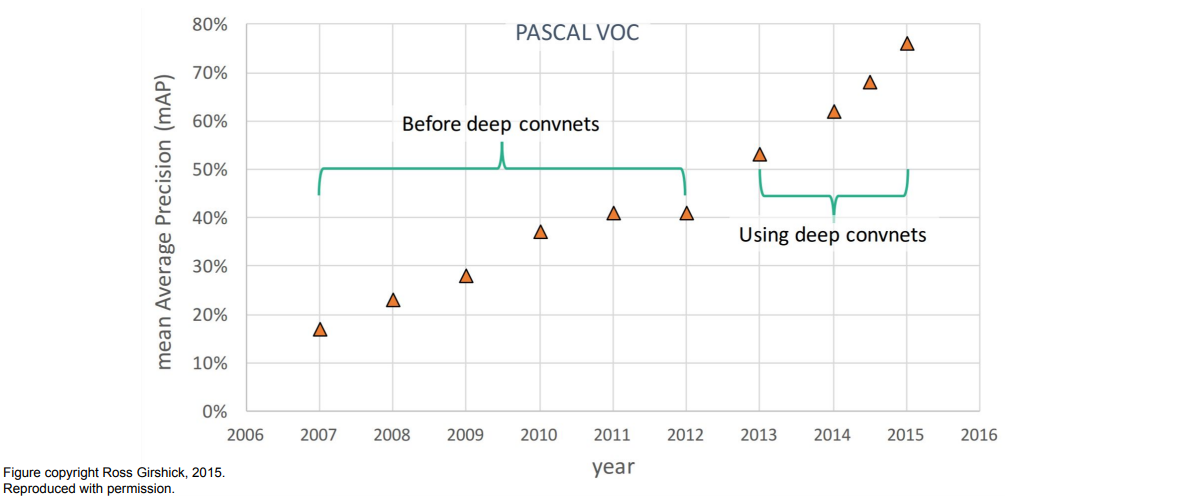
\includegraphics[width=\figwidth]{Object_Detect_impact_of_DL}
	\slcaption{
		Mean average precission (mAP) of object detection before and after using deep learning techniques. (\textcite{Fei-Fei2017}, Slide 54).
		\label{fig:Object_Detect_impact_of_DL}}
\end{figure}

\section{Challenges}






\chapter{Related work}





\chapter{Methods}

\section{}


\chapter{Time frame}


\chapter{Conclusion}


% Acronym definitions
%TODO Add acronym definitions produced by acronyms2glossary.py 




\glsaddall
\printglossaries

\printbibliography

\end{document}